% Options for packages loaded elsewhere
\PassOptionsToPackage{unicode}{hyperref}
\PassOptionsToPackage{hyphens}{url}
%
\documentclass[
]{book}
\usepackage{amsmath,amssymb}
\usepackage{lmodern}
\usepackage{ifxetex,ifluatex}
\ifnum 0\ifxetex 1\fi\ifluatex 1\fi=0 % if pdftex
  \usepackage[T1]{fontenc}
  \usepackage[utf8]{inputenc}
  \usepackage{textcomp} % provide euro and other symbols
\else % if luatex or xetex
  \usepackage{unicode-math}
  \defaultfontfeatures{Scale=MatchLowercase}
  \defaultfontfeatures[\rmfamily]{Ligatures=TeX,Scale=1}
\fi
% Use upquote if available, for straight quotes in verbatim environments
\IfFileExists{upquote.sty}{\usepackage{upquote}}{}
\IfFileExists{microtype.sty}{% use microtype if available
  \usepackage[]{microtype}
  \UseMicrotypeSet[protrusion]{basicmath} % disable protrusion for tt fonts
}{}
\makeatletter
\@ifundefined{KOMAClassName}{% if non-KOMA class
  \IfFileExists{parskip.sty}{%
    \usepackage{parskip}
  }{% else
    \setlength{\parindent}{0pt}
    \setlength{\parskip}{6pt plus 2pt minus 1pt}}
}{% if KOMA class
  \KOMAoptions{parskip=half}}
\makeatother
\usepackage{xcolor}
\IfFileExists{xurl.sty}{\usepackage{xurl}}{} % add URL line breaks if available
\IfFileExists{bookmark.sty}{\usepackage{bookmark}}{\usepackage{hyperref}}
\hypersetup{
  pdftitle={AMAT- Ciencia de Datos y Machine Learning 2},
  pdfauthor={Karina Lizette Gamboa Puente; Oscar Arturo Bringas López},
  hidelinks,
  pdfcreator={LaTeX via pandoc}}
\urlstyle{same} % disable monospaced font for URLs
\usepackage{color}
\usepackage{fancyvrb}
\newcommand{\VerbBar}{|}
\newcommand{\VERB}{\Verb[commandchars=\\\{\}]}
\DefineVerbatimEnvironment{Highlighting}{Verbatim}{commandchars=\\\{\}}
% Add ',fontsize=\small' for more characters per line
\usepackage{framed}
\definecolor{shadecolor}{RGB}{248,248,248}
\newenvironment{Shaded}{\begin{snugshade}}{\end{snugshade}}
\newcommand{\AlertTok}[1]{\textcolor[rgb]{0.94,0.16,0.16}{#1}}
\newcommand{\AnnotationTok}[1]{\textcolor[rgb]{0.56,0.35,0.01}{\textbf{\textit{#1}}}}
\newcommand{\AttributeTok}[1]{\textcolor[rgb]{0.77,0.63,0.00}{#1}}
\newcommand{\BaseNTok}[1]{\textcolor[rgb]{0.00,0.00,0.81}{#1}}
\newcommand{\BuiltInTok}[1]{#1}
\newcommand{\CharTok}[1]{\textcolor[rgb]{0.31,0.60,0.02}{#1}}
\newcommand{\CommentTok}[1]{\textcolor[rgb]{0.56,0.35,0.01}{\textit{#1}}}
\newcommand{\CommentVarTok}[1]{\textcolor[rgb]{0.56,0.35,0.01}{\textbf{\textit{#1}}}}
\newcommand{\ConstantTok}[1]{\textcolor[rgb]{0.00,0.00,0.00}{#1}}
\newcommand{\ControlFlowTok}[1]{\textcolor[rgb]{0.13,0.29,0.53}{\textbf{#1}}}
\newcommand{\DataTypeTok}[1]{\textcolor[rgb]{0.13,0.29,0.53}{#1}}
\newcommand{\DecValTok}[1]{\textcolor[rgb]{0.00,0.00,0.81}{#1}}
\newcommand{\DocumentationTok}[1]{\textcolor[rgb]{0.56,0.35,0.01}{\textbf{\textit{#1}}}}
\newcommand{\ErrorTok}[1]{\textcolor[rgb]{0.64,0.00,0.00}{\textbf{#1}}}
\newcommand{\ExtensionTok}[1]{#1}
\newcommand{\FloatTok}[1]{\textcolor[rgb]{0.00,0.00,0.81}{#1}}
\newcommand{\FunctionTok}[1]{\textcolor[rgb]{0.00,0.00,0.00}{#1}}
\newcommand{\ImportTok}[1]{#1}
\newcommand{\InformationTok}[1]{\textcolor[rgb]{0.56,0.35,0.01}{\textbf{\textit{#1}}}}
\newcommand{\KeywordTok}[1]{\textcolor[rgb]{0.13,0.29,0.53}{\textbf{#1}}}
\newcommand{\NormalTok}[1]{#1}
\newcommand{\OperatorTok}[1]{\textcolor[rgb]{0.81,0.36,0.00}{\textbf{#1}}}
\newcommand{\OtherTok}[1]{\textcolor[rgb]{0.56,0.35,0.01}{#1}}
\newcommand{\PreprocessorTok}[1]{\textcolor[rgb]{0.56,0.35,0.01}{\textit{#1}}}
\newcommand{\RegionMarkerTok}[1]{#1}
\newcommand{\SpecialCharTok}[1]{\textcolor[rgb]{0.00,0.00,0.00}{#1}}
\newcommand{\SpecialStringTok}[1]{\textcolor[rgb]{0.31,0.60,0.02}{#1}}
\newcommand{\StringTok}[1]{\textcolor[rgb]{0.31,0.60,0.02}{#1}}
\newcommand{\VariableTok}[1]{\textcolor[rgb]{0.00,0.00,0.00}{#1}}
\newcommand{\VerbatimStringTok}[1]{\textcolor[rgb]{0.31,0.60,0.02}{#1}}
\newcommand{\WarningTok}[1]{\textcolor[rgb]{0.56,0.35,0.01}{\textbf{\textit{#1}}}}
\usepackage{longtable,booktabs,array}
\usepackage{calc} % for calculating minipage widths
% Correct order of tables after \paragraph or \subparagraph
\usepackage{etoolbox}
\makeatletter
\patchcmd\longtable{\par}{\if@noskipsec\mbox{}\fi\par}{}{}
\makeatother
% Allow footnotes in longtable head/foot
\IfFileExists{footnotehyper.sty}{\usepackage{footnotehyper}}{\usepackage{footnote}}
\makesavenoteenv{longtable}
\usepackage{graphicx}
\makeatletter
\def\maxwidth{\ifdim\Gin@nat@width>\linewidth\linewidth\else\Gin@nat@width\fi}
\def\maxheight{\ifdim\Gin@nat@height>\textheight\textheight\else\Gin@nat@height\fi}
\makeatother
% Scale images if necessary, so that they will not overflow the page
% margins by default, and it is still possible to overwrite the defaults
% using explicit options in \includegraphics[width, height, ...]{}
\setkeys{Gin}{width=\maxwidth,height=\maxheight,keepaspectratio}
% Set default figure placement to htbp
\makeatletter
\def\fps@figure{htbp}
\makeatother
\setlength{\emergencystretch}{3em} % prevent overfull lines
\providecommand{\tightlist}{%
  \setlength{\itemsep}{0pt}\setlength{\parskip}{0pt}}
\setcounter{secnumdepth}{5}
\usepackage{booktabs}
\ifluatex
  \usepackage{selnolig}  % disable illegal ligatures
\fi
\usepackage[]{natbib}
\bibliographystyle{apalike}

\title{AMAT- Ciencia de Datos y Machine Learning 2}
\author{Karina Lizette Gamboa Puente \and Oscar Arturo Bringas López}
\date{}

\begin{document}
\maketitle

{
\setcounter{tocdepth}{1}
\tableofcontents
}
\hypertarget{bienvenida}{%
\chapter{BIENVENIDA}\label{bienvenida}}

\hypertarget{objetivo}{%
\section{Objetivo}\label{objetivo}}

Desarrollar conocimiento y habilidades para implementar modelos complejos de Machine Learning a través de un flujo de trabajo limpio, ordenado y sistematizado a mediante las librerías en \emph{R} más novedosas que han sido desarrolladas hasta el momento. Al finalizar este curso, el participante será capáz de combinar distintas clases de modelos para dar una solución compleja y precisa a problemas predictivos. Aprenderá a cuantificar los problemas éticos asociados al sesgo o inequidad producidos por modelos de machine learning, así como su interpretación en el mundo productivo. Finalmente, se estudiará la manera de desarrollar un diseño de experimento para implementarse en el ámbito empresarial de modo que el participante pueda tomar mejores decisiones para contribuir en su ambiente laboral.

\textbf{Se asume que el alumno tiene conocimientos generales de estadística, bases matemáticas y de programación básica en R y que cuenta con los conocimientos teóricos básicos de machine learning y prácticos con tidymodels.}

\hypertarget{quienes-somos}{%
\section{¿Quienes somos?}\label{quienes-somos}}

\textbf{ACT. ARTURO BRINGAS}

\textbf{LinkedIn:} \href{https://www.linkedin.com/in/arturo-bringas/}{arturo-bringas}
\textbf{Email:} \href{mailto:act.arturo.b@ciencias.unam.mx}{\nolinkurl{act.arturo.b@ciencias.unam.mx}}

Actuario, egresado de la Facultad de Ciencias y Maestría en Ciencia de Datos, ITAM.
Experiencia en modelos predictivos y de clasificación de machine learning aplicado a seguros, deportes y movilidad internacional. Es jefe de departamento en Investigación Aplicada y Opinión de la UNAM, donde realiza estudios estadísticos de impacto social. Es consultor para empresas y organizaciones como GNP, El Universal, UNAM, Sinnia, la Organización de las Naciones Unidas Contra la Droga y el Delito (UNODC), entre otros. Actualmente es profesor de \emph{ciencia de datos y machine learning} en AMAT y se desempeña como consultor independiente en diferentes proyectos contribuyendo a empresas en temas de machine learning, estadística, series de tiempo, visualización de datos y análisis geoespacial.

\begin{center}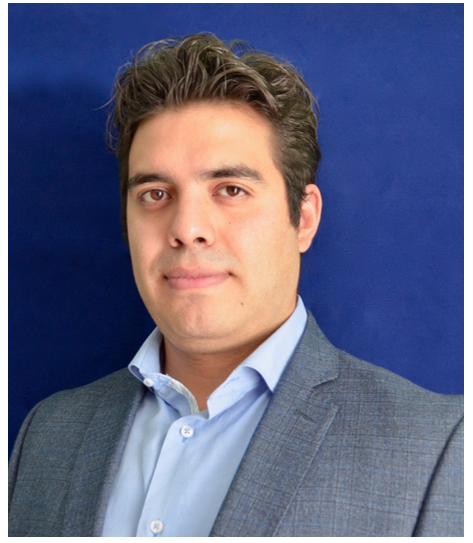
\includegraphics[width=6.57in]{img/00-presentacion/arturo} \end{center}

\textbf{ACT. KARINA LIZETTE GAMBOA}

\textbf{LinkedIn:} \href{https://www.linkedin.com/in/kalizzygam/}{KaLizzyGam}
\textbf{Email:} \href{mailto:lizzygamboa@ciencias.unam.mx}{\nolinkurl{lizzygamboa@ciencias.unam.mx}}

Actuaria, egresada de la Facultad de Ciencias, UNAM, candidata a Maestra en
Ciencia de Datos por el ITAM.

Experiencia en áreas de analítica predictiva e inteligencia del negocio. Lead y Senior
Data Scientist en consultoría en diferentes sectores como tecnología, asegurador,
financiero y bancario. Experta en entendimiento de negocio para la correcta
implementación de algoritmos de inteligencia y explotación de datos.
Actualmente se desarrolla como Arquitecta de Soluciones Analíticas en Merama,
startup mexicana clasificada como uno de los nuevos unicornios de Latinoamérica.
Senior Data Science en CLOSTER y como profesora del diplomado de Metodología
de la Investigación Social por la UNAM así como instructora de cursos de Ciencia de
Datos en AMAT.

Empresas anteriores: GNP, Activer Banco y Casa de Bolsa, PlayCity Casinos,
RakenDataGroup Consulting, entre otros.

\begin{center}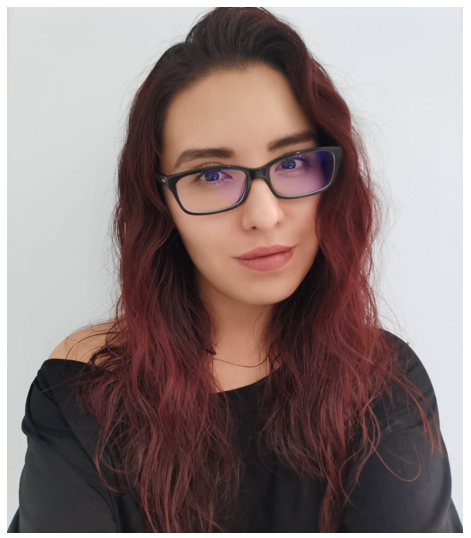
\includegraphics[width=6.54in]{img/00-presentacion/lizzy} \end{center}

\hypertarget{ciencia-de-datos-en-r}{%
\section{Ciencia de Datos en R}\label{ciencia-de-datos-en-r}}

\begin{center}
\includegraphics[width=28.53in]{img/00-presentacion/DataScienceVerse} \end{center}

\hypertarget{estructura-del-curso-actual}{%
\section{Estructura del curso actual}\label{estructura-del-curso-actual}}

\hypertarget{alcances-del-curso}{%
\subsection{Alcances del curso}\label{alcances-del-curso}}

Al finalizar el módulo, el participante sabrá plantear un proyecto de ciencia de datos, desde sus requerimientos hasta sus implementación comercial. Sabrá crear flujos de trabajo limpios y ordenados para crear poderosos modelos de Machine Learning. Podrá comparar múltiples modelos y seleccionar el que más aportación realice a su negocio considerando la ética alrededor del sesgo e inequidad producida por modelos. Profundizará su conocimiento en la interpretación de modelos complejos y aprenderá a cuantificar el beneficio comercial de la implementación de modelos.

\textbf{Requisitos:}

\begin{quote}
Computadora con al menos 4Gb Ram.
\end{quote}

\begin{quote}
Instalación de R con al menos versión 4.1.0
\end{quote}

\begin{quote}
Instalación de Rstudio con al menos versión 1.4
\end{quote}

\begin{quote}
Data Science \& Machine Learning (Aprendizaje Supervisado I)
\end{quote}

\textbf{Temario:}

\textbf{1.- Machine Learning (10 HRS)}

\begin{itemize}
\tightlist
\item
  Regresión polinomial
\item
  Regresión con CPA
\item
  Imputación
\item
  SVM
\item
  Boosting
\end{itemize}

\textbf{2. Flujos de trabajo y ensamblajes (8 HRS)}

\begin{itemize}
\tightlist
\item
  Pipelines
\item
  Workflowsets
\item
  Comparación de modelos
\item
  Stacking
\end{itemize}

\textbf{3. Sesgo e inequidad de modelos (4 HRS)}

\begin{itemize}
\tightlist
\item
  Cuantificación de sesgo
\item
  Cuantificación de inequidad
\end{itemize}

\textbf{4. Interpretación de modelos (4 HRS)}

\begin{itemize}
\tightlist
\item
  LIME
\item
  ghv
\end{itemize}

\textbf{5. Aplicación a negocios (6 HRS)}

\begin{itemize}
\tightlist
\item
  Diseño de experimentos en campañas de retención
\item
  Valuación de implementación de modelos
\end{itemize}

\hypertarget{duraciuxf3n-y-evaluaciuxf3n-del-curso}{%
\section{Duración y evaluación del curso}\label{duraciuxf3n-y-evaluaciuxf3n-del-curso}}

\begin{itemize}
\item
  El programa tiene una duración de 32 hrs.
\item
  Las clases serán impartidas los días domingo, de 9:00 am a 1:00 pm
\item
  Serán asignados ejercicios que el participante deberá resolver entre una semana y otra.
\item
  Al final del curso se solicitará un proyecto final, el cual \textbf{deberá ser entregado para ser acreedor a la constancia de participación}.
\end{itemize}

\hypertarget{recursos-y-dinuxe1mica-de-clase}{%
\section{Recursos y dinámica de clase}\label{recursos-y-dinuxe1mica-de-clase}}

En esta clase estaremos usando:

\begin{itemize}
\tightlist
\item
  R \href{https://cran.r-project.org/}{da click aquí si aún no lo descargas}
\item
  RStudio \href{https://www.rstudio.com/products/rstudio/download/}{da click aquí también}
\item
  Miro \href{https://miro.com/welcomeonboard/c3huendzNURhRUVGbHlsWGVFYlBBMXRaSncybXRrbjBRU2R5WWg2eDFKUXY1VlJ1SGJFdmc4ZmRuWEgwcllpenwzMDc0NDU3MzYxMzQwNDIyODEy?invite_link_id=152058640259}{úsame}
\item
  Zoom \href{https://us02web.zoom.us/j/5155440751?pwd=YzJCOGF0VnlZdlZlS0Fpc3MvZEhadz09}{Clases}

  \begin{itemize}
  \tightlist
  \item
    Pulgar arriba: Voy bien, estoy entendiendo!
  \item
    Pulgar abajo: Eso no quedó muy claro
  \item
    Mano arriba: Quiero participar/preguntar ó Ya estoy listo para iniciar
  \end{itemize}
\item
  Grupo de WhatsApp \href{https://chat.whatsapp.com/KUbqIk8Cqu42zkXffIgUQQ}{El chismecito está aquí}
\item
  \href{https://drive.google.com/drive/folders/1IblKYfDpSjV89FBT3c-PafOiD4wW7UrD?usp=sharing}{Google Drive}
\item
  Notas de clase \href{https://acturio.github.io/amt22_03intro2mls2/}{Revisame si quieres aprender}
\item
  Documento del taller de \href{https://docs.google.com/spreadsheets/d/1hCRt00nYyZvbkfi9yOMRSR0R30lPRtKzaNKKlgAE78M/edit?usp=sharing}{Scoping}.
\end{itemize}

\hypertarget{supervised-machine-learning}{%
\chapter{Supervised Machine Learning}\label{supervised-machine-learning}}

En este curso analizaremos distintos métodos de machine learning que permitirán predecir una respuesta numérica o categórica. Usaremos el lenguaje de programación \emph{R}.

\hypertarget{support-vector-machine-svm}{%
\section{Support Vector Machine (SVM)}\label{support-vector-machine-svm}}

Support vector machine, llamadas SVM, son un algoritmo de aprendizaje supervisado que se puede utilizar para problemas de clasificación y regresión. Se utiliza para conjuntos de datos más pequeños, ya que tarda demasiado en procesarse.

\begin{center}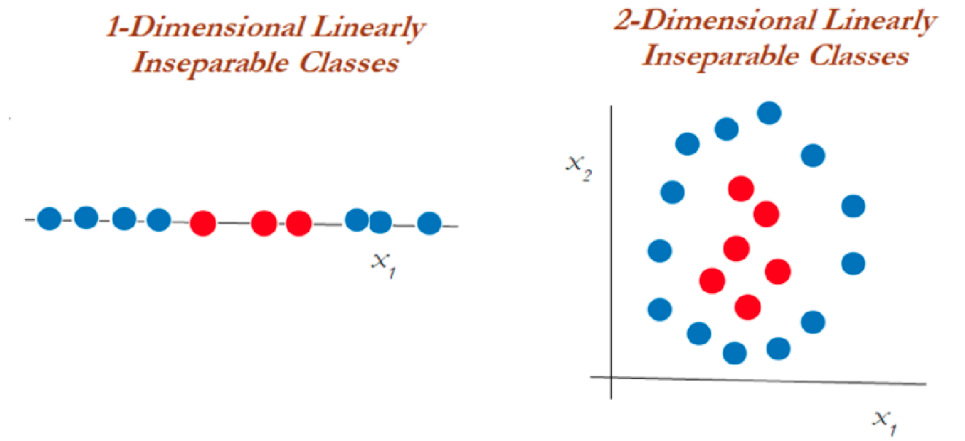
\includegraphics[width=800pt,height=400pt]{img/03-svm/01_inseparable_classes} \end{center}

El principal objetivo de esta técnica es encontrar el \textbf{Hiperplano de Separación Óptima}, también conocido como \emph{Boundary Decision}, el cual separa a las clases involucradas.

Para entender este algoritmo es necesario entender 3 conceptos principales:

\begin{quote}
\begin{enumerate}
\def\labelenumi{\arabic{enumi}.}
\tightlist
\item
  Maximum margin classifiers
\end{enumerate}
\end{quote}

\begin{quote}
\begin{enumerate}
\def\labelenumi{\arabic{enumi}.}
\setcounter{enumi}{1}
\tightlist
\item
  Support vector classifiers
\end{enumerate}
\end{quote}

\begin{quote}
\begin{enumerate}
\def\labelenumi{\arabic{enumi}.}
\setcounter{enumi}{2}
\tightlist
\item
  Support vector machines
\end{enumerate}
\end{quote}

Estudiemos cada uno de estos principios.

\hypertarget{maximum-margin-classifier}{%
\subsection{Maximum Margin Classifier}\label{maximum-margin-classifier}}

A menudo se generalizan con máquinas de vectores de soporte, pero SVM tiene muchos más parámetros en comparación. El \emph{clasificador de margen máximo} considera un hiperplano con ancho de separación máxima para clasificar los datos. Sin embargo, se pueden dibujar infinitos hiperplanos en un conjunto de datos por lo que es importante elegir el hiperplano ideal para la clasificación.

En un espacio \emph{n-dimensional}, un hiperplano es un subespacio de la dimensión n-1. Es decir, si los datos tienen un espacio bidimensional, entonces el hiperplano puede ser una línea recta que divide el espacio de datos en dos mitades y pasa por la siguiente ecuacion:

\[\beta_0 + \beta_1X_1 + \beta_2X_2=0\]

Las observaciones que caen en el hiperplano sigue la ecuación anterior. Las observaciones que caen en la región por encima o por debajo del hiperplano sigue las siguientes ecuaciones:

\[\beta_0 + \beta_1X_1 + \beta_2X_2>0\]

\[\beta_0 + \beta_1X_1 + \beta_2X_2<0\]

El clasificador de margen máximo a menudo falla en la situación de casos no separables en los que no puede asignar un hiperplano diferente para clasificar datos no separables. Para tales casos, un clasificador de vectores de soporte viene al rescate.

\begin{center}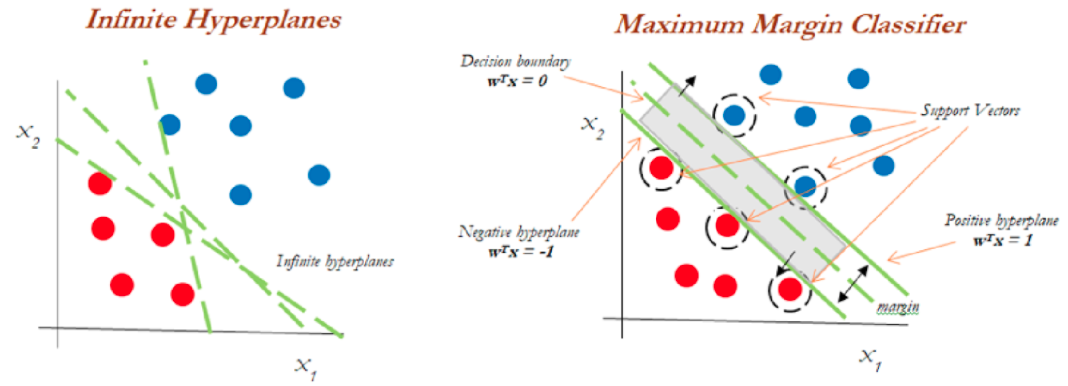
\includegraphics[width=900pt,height=380pt]{img/03-svm/02_maximum_margin_classifier} \end{center}

Del diagrama anterior, podemos suponer infinitos hiperplanos (izquierda). El clasificador de margen máximo viene con un solo hiperplano que divide los datos como en la gráfica de la derecha. \textbf{Los datos que tocan los hiperplanos positivo y negativo se denominan vectores de soporte}.

\hypertarget{support-vector-classifiers}{%
\subsection{Support Vector Classifiers}\label{support-vector-classifiers}}

\textbf{Los vectores de soporte son las observaciones que están más cerca del hiperplano e influyen en la posición y orientación del hiperplano}. Este tipo de clasificador puede considerarse como una versión extendida del clasificador de margen máximo. Cuando tratamos con datos de la vida real, encontramos que la mayoría de las observaciones están en clases superpuestas. Es por eso que se implementan clasificadores de vectores de soporte.

Usando estos vectores de soporte, maximizamos el margen del clasificador. Eliminar los vectores de soporte cambiará la posición del hiperplano. Estos son los puntos que nos ayudan a construir nuestro \emph{SVM}. Consideremos un \textbf{parámetro de ajuste C}. En este clasificador, el alto valor de \emph{C} puede darnos un modelo robusto. Un valor más bajo de \emph{C} nos da un modelo flexible. Entendamos con el siguiente diagrama.

\begin{center}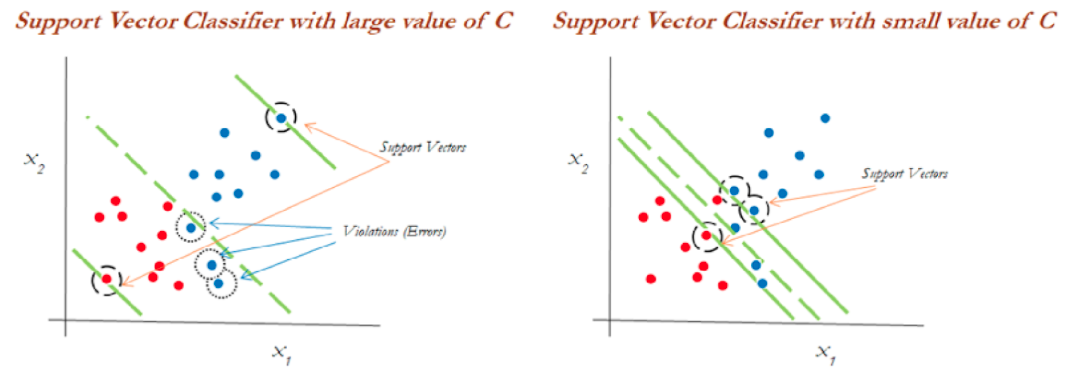
\includegraphics[width=900pt,height=380pt]{img/03-svm/03_support_vector_classifier} \end{center}

Podemos ver en el gráfico de la izquierda que los valores más altos de \emph{C} generaron más errores que se consideran una \textbf{violación o infracción}. El diagrama de la derecha muestra un valor más bajo de \emph{C} y no brinda suficientes posibilidades de infracción al reducir el ancho del margen.

\hypertarget{support-vector-machine}{%
\subsection{Support Vector Machine}\label{support-vector-machine}}

El enfoque de la máquina de vectores de soporte se considera durante una decisión no lineal y los datos no son separables por un clasificador de vectores de soporte, independientemente de la función de costo.

Cuando es casi imposible separar clases de manera no lineal, aplicamos el truco llamado \textbf{truco del kernel} el cual ayuda a manejar la separación de los datos.

\begin{center}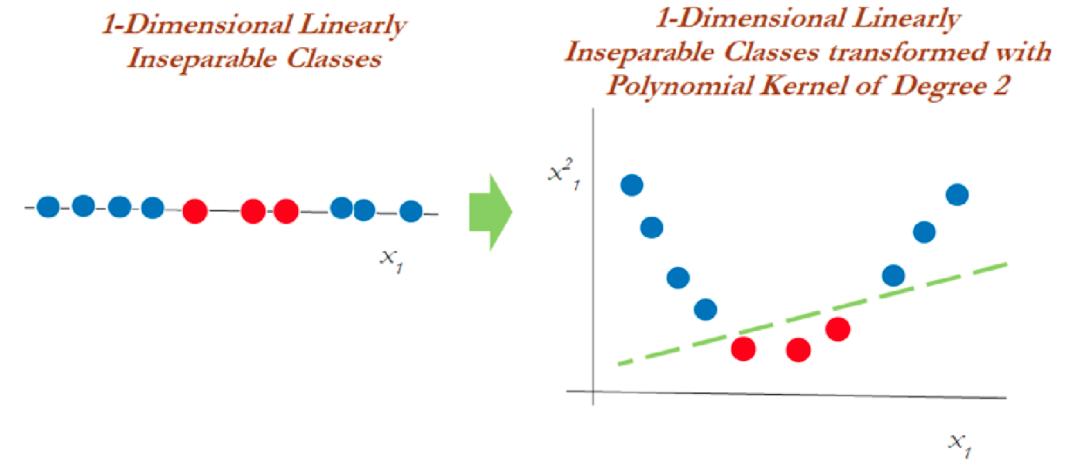
\includegraphics[width=900pt,height=380pt]{img/03-svm/04_polinomial_kernel_plot} \end{center}

En el gráfico anterior, los datos que eran inseparables en una dimensión se separaron una vez que se transformaron a un espacio de dos dimensiones después de aplicar una \textbf{transformación mediante kernel polinomial de segundo grado}. Ahora veamos cómo manejar los datos bidimensionales linealmente inseparables.

\begin{center}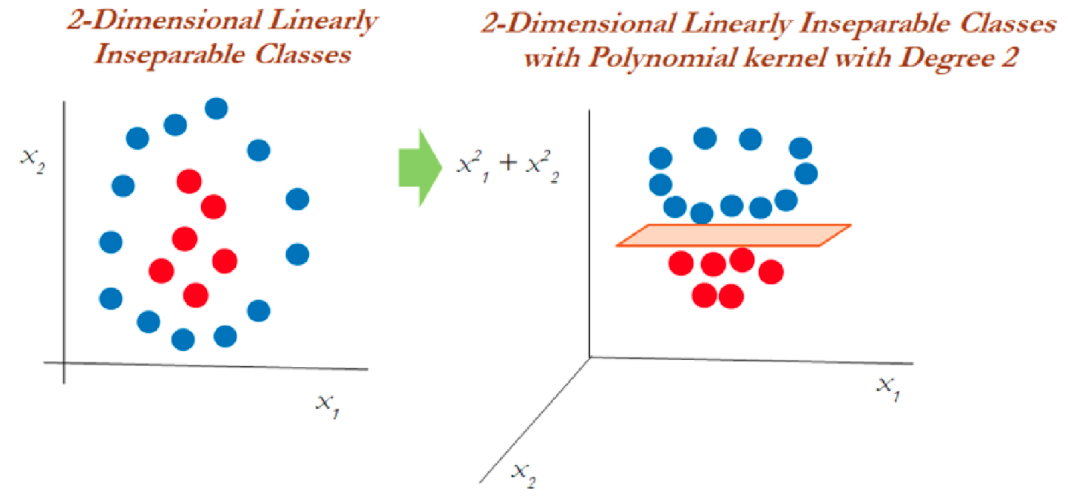
\includegraphics[width=900pt,height=380pt]{img/03-svm/05_kernel_polinomial_plot2} \end{center}

En datos bidimensionales, el núcleo polinomial de segundo grado se aplica utilizando un plano lineal después de transformarlo a dimensiones superiores.

\hypertarget{el-truco-del-kernel}{%
\subsection{El truco del Kernel}\label{el-truco-del-kernel}}

Las funciones Kernel son métodos con los que se utilizan clasificadores lineales como \emph{SVM} para clasificar puntos de datos separables no linealmente. Esto se hace representando los puntos de datos en un espacio de mayor dimensión que su original. Por ejemplo, los datos 1D se pueden representar como datos 2D en el espacio, los datos 2D se pueden representar como datos 3D, etcétera.

El truco del kernel ofrece una \textbf{forma de calcular las relaciones entre los puntos de datos} utilizando funciones del kernel y representar los datos de una manera más eficiente con menos cómputo. Los modelos que utilizan esta técnica se denominan \textbf{``modelos kernelizados''}.

\begin{center}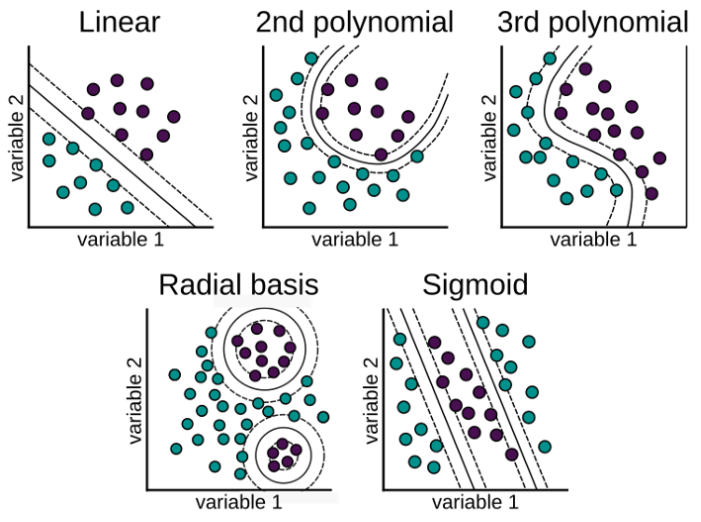
\includegraphics[width=700pt,height=500pt]{img/03-svm/06_kernels} \end{center}

Hay varias funciones que utiliza SVM para realizar esta tarea. Algunos de los más comunes son:

\begin{enumerate}
\def\labelenumi{\arabic{enumi}.}
\tightlist
\item
  \textbf{El núcleo lineal:} Se utiliza para datos lineales. Esto simplemente representa los puntos de datos usando una relación lineal.
\end{enumerate}

\[K(x, y)=(x^T \cdot y)\]
\[f(x)=w^T \cdot x + b\]
Esta formulación se presenta como solución al problema de optimización sobre w:

\[min_{w\in R^d} \parallel w \parallel ^2+ C\sum_{i}^{N}{max(0, 1-y_if(x_i))}\]
\[s.a. \quad y_i(w^T x_i+b) \geq 1 - max(0, 1-y_if(x_i))\]

\begin{enumerate}
\def\labelenumi{\arabic{enumi}.}
\setcounter{enumi}{1}
\tightlist
\item
  \textbf{Función de núcleo polinomial:} Transforma los puntos de datos mediante el \textbf{uso del producto escalar} y la transformación de los datos en una ``dimensión \emph{n}'', \emph{n} podría ser cualquier valor de 2, 3, etcétera, es decir, la transformación será un producto al cuadrado o superior. Por lo tanto, representar datos en un espacio de mayor dimensión utilizando los nuevos puntos transformados.
\end{enumerate}

\[K(x, y)=(c+ x^T \cdot y)^p\]

Cuando se emplea \(p=1\) y \(c=0\), el resultado es el mismo que el de un kernel lineal. Si \(p>1\), se generan límites de decisión no lineales, aumentando la no linealidad a medida que aumenta \emph{p}. No suele ser recomendable emplear valores de \emph{p} mayores 5 por problemas de \textbf{overfitting}.

\begin{center}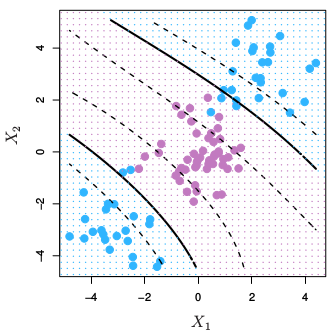
\includegraphics[width=400pt,height=400pt]{img/03-svm/3-15-1-poli} \end{center}

\begin{enumerate}
\def\labelenumi{\arabic{enumi}.}
\setcounter{enumi}{2}
\tightlist
\item
  \textbf{La función de base radial (RBF):} Esta función se comporta como un ``modelo de vecino más cercano ponderado''. Transforma los datos representándolos en dimensiones infinitas,
\end{enumerate}

La función Radial puede ser de Gauss o de Laplace. Esto depende de un hiperparámetro conocido como gamma \(\gamma\). Cuanto menor sea el valor del hiperparámetro, menor será el sesgo y mayor la varianza. Mientras que un valor más alto de hiperparámetro da un sesgo más alto y menor varianza. Este es el núcleo más utilizado.

\[K(x, y)=exp(-\gamma \parallel x - y\parallel^2)=exp(-\frac{\parallel x-y \parallel ^2}{2\sigma²})\]
\[f(x)=w^T \cdot \phi(x) + b\]
Se realiza un mapeo de x a \(\phi(x)\) en donde los datos son separables

\begin{center}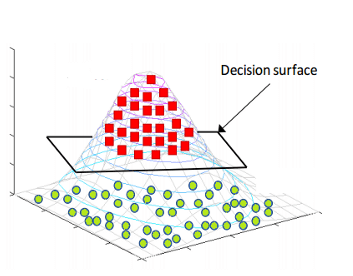
\includegraphics[width=400pt,height=400pt]{img/03-svm/svm_radial} \end{center}

Es recomendable probar el kernel \textbf{RBF}. Este kernel tiene dos ventajas: que solo tiene dos hiperparámetros que optimizar (\(\gamma\) y la penalización \(C\) común a todos los SVM) y que su flexibilidad puede ir desde un clasificador lineal a uno muy complejo.

\begin{enumerate}
\def\labelenumi{\arabic{enumi}.}
\setcounter{enumi}{3}
\tightlist
\item
  \textbf{La función sigmoide:} También conocida como función tangente hiperbólica (Tanh), encuentra más aplicación en redes neuronales como función de activación. Esta función se utiliza en la clasificación de imágenes.
\end{enumerate}

\[K(x, y)= tanh(\kappa x\cdot y-\delta)\]

¿Por qué se llama un ``truco del kernel''? \emph{SVM} vuelve a representar hábilmente los puntos de datos no lineales utilizando cualquiera de las funciones del kernel de una manera que parece que los datos se han transformado, luego encuentra el hiperplano de separación óptimo. Sin embargo, en realidad, los puntos de datos siguen siendo los mismos, en realidad no se han transformado. Es por eso que se llama un `truco del kernel'.

\hypertarget{ventajas-y-desventajas}{%
\subsection{Ventajas y desventajas}\label{ventajas-y-desventajas}}

\textbf{Ventajas}

\begin{itemize}
\item
  Es un modelo que ajusta bien con pocos datos
\item
  Son flexibles en datos no estructurados, estructurados y semiestructurados.
\item
  La función Kernel alivia las complejidades en casi cualquier tipo de datos.
\item
  Se observa menos sobreajuste en comparación con otros modelos.
\end{itemize}

\textbf{Desventajas}

\begin{itemize}
\item
  El tiempo de entrenamiento es mayor cuando se calculan grandes conjuntos de datos.
\item
  Los hiperparámetros suelen ser un desafío al interpretar su impacto.
\item
  La interpretación general es difícil (black box).
\end{itemize}

\hypertarget{ajuste-del-modelo-con-r}{%
\subsection{Ajuste del modelo con R}\label{ajuste-del-modelo-con-r}}

Usaremos las recetas antes implementadas para ajustar tanto el modelo de regresión como el de clasificación. Exploraremos un conjunto de hiperparámetros para elegir el mejor modelo.

Recordemos que es importante separar los datos de entrenamiento y prueba, así como sub-particionar en fold a los datos de entrenamiento para realizar diferentes pruebas con distintas parametrizaciones de los modelos. Finalmente, calcularemos el error promedio y los mejores hiperparámetros a implementar.

\begin{Shaded}
\begin{Highlighting}[]
\FunctionTok{library}\NormalTok{(tidymodels)}

\FunctionTok{data}\NormalTok{(ames)}

\FunctionTok{set.seed}\NormalTok{(}\DecValTok{4595}\NormalTok{)}
\NormalTok{ames\_split }\OtherTok{\textless{}{-}} \FunctionTok{initial\_split}\NormalTok{(ames, }\AttributeTok{prop =} \FloatTok{0.75}\NormalTok{)}
\NormalTok{ames\_train }\OtherTok{\textless{}{-}} \FunctionTok{training}\NormalTok{(ames\_split)}
\NormalTok{ames\_test  }\OtherTok{\textless{}{-}} \FunctionTok{testing}\NormalTok{(ames\_split)}
\NormalTok{ames\_folds}\OtherTok{\textless{}{-}} \FunctionTok{vfold\_cv}\NormalTok{(ames\_train)}
\end{Highlighting}
\end{Shaded}

Contando con datos de entrenamiento, procedemos a realizar el feature engineering para extraer las mejores características que permitirán realizar las estimaciones en el modelo.

\begin{Shaded}
\begin{Highlighting}[]
\NormalTok{receta\_casas }\OtherTok{\textless{}{-}} \FunctionTok{recipe}\NormalTok{(Sale\_Price }\SpecialCharTok{\textasciitilde{}}\NormalTok{ . , }\AttributeTok{data =}\NormalTok{ ames\_train) }\SpecialCharTok{\%\textgreater{}\%}
  \FunctionTok{step\_unknown}\NormalTok{(Alley) }\SpecialCharTok{\%\textgreater{}\%}
  \FunctionTok{step\_rename}\NormalTok{(}\AttributeTok{Year\_Remod =}\NormalTok{ Year\_Remod\_Add) }\SpecialCharTok{\%\textgreater{}\%} 
  \FunctionTok{step\_rename}\NormalTok{(}\AttributeTok{ThirdSsn\_Porch =}\NormalTok{ Three\_season\_porch) }\SpecialCharTok{\%\textgreater{}\%} 
  \FunctionTok{step\_ratio}\NormalTok{(Bedroom\_AbvGr, }\AttributeTok{denom =} \FunctionTok{denom\_vars}\NormalTok{(Gr\_Liv\_Area)) }\SpecialCharTok{\%\textgreater{}\%} 
  \FunctionTok{step\_mutate}\NormalTok{(}
    \AttributeTok{Age\_House =}\NormalTok{ Year\_Sold }\SpecialCharTok{{-}}\NormalTok{ Year\_Remod,}
    \AttributeTok{TotalSF   =}\NormalTok{ Gr\_Liv\_Area }\SpecialCharTok{+}\NormalTok{ Total\_Bsmt\_SF,}
    \AttributeTok{AvgRoomSF   =}\NormalTok{ Gr\_Liv\_Area }\SpecialCharTok{/}\NormalTok{ TotRms\_AbvGrd,}
    \AttributeTok{Pool =} \FunctionTok{if\_else}\NormalTok{(Pool\_Area }\SpecialCharTok{\textgreater{}} \DecValTok{0}\NormalTok{, }\DecValTok{1}\NormalTok{, }\DecValTok{0}\NormalTok{),}
    \AttributeTok{Exter\_Cond =}\NormalTok{ forcats}\SpecialCharTok{::}\FunctionTok{fct\_collapse}\NormalTok{(Exter\_Cond, }\AttributeTok{Good =} \FunctionTok{c}\NormalTok{(}\StringTok{"Typical"}\NormalTok{, }\StringTok{"Good"}\NormalTok{, }\StringTok{"Excellent"}\NormalTok{))) }\SpecialCharTok{\%\textgreater{}\%} 
  \FunctionTok{step\_relevel}\NormalTok{(Exter\_Cond, }\AttributeTok{ref\_level =} \StringTok{"Good"}\NormalTok{) }\SpecialCharTok{\%\textgreater{}\%} 
  \FunctionTok{step\_normalize}\NormalTok{(}\FunctionTok{all\_predictors}\NormalTok{(), }\SpecialCharTok{{-}}\FunctionTok{all\_nominal}\NormalTok{()) }\SpecialCharTok{\%\textgreater{}\%}
  \FunctionTok{step\_dummy}\NormalTok{(}\FunctionTok{all\_nominal}\NormalTok{()) }\SpecialCharTok{\%\textgreater{}\%} 
  \FunctionTok{step\_interact}\NormalTok{(}\SpecialCharTok{\textasciitilde{}}\NormalTok{ Second\_Flr\_SF}\SpecialCharTok{:}\NormalTok{First\_Flr\_SF) }\SpecialCharTok{\%\textgreater{}\%} 
  \FunctionTok{step\_interact}\NormalTok{(}\SpecialCharTok{\textasciitilde{}} \FunctionTok{matches}\NormalTok{(}\StringTok{"Bsmt\_Cond"}\NormalTok{)}\SpecialCharTok{:}\NormalTok{TotRms\_AbvGrd) }\SpecialCharTok{\%\textgreater{}\%} 
  \FunctionTok{step\_rm}\NormalTok{(}
\NormalTok{    First\_Flr\_SF, Second\_Flr\_SF, Year\_Remod,}
\NormalTok{    Bsmt\_Full\_Bath, Bsmt\_Half\_Bath, }
\NormalTok{    Kitchen\_AbvGr, BsmtFin\_Type\_1\_Unf, }
\NormalTok{    Total\_Bsmt\_SF, Kitchen\_AbvGr, Pool\_Area, }
\NormalTok{    Gr\_Liv\_Area, Sale\_Type\_Oth, Sale\_Type\_VWD}
\NormalTok{  ) }\SpecialCharTok{\%\textgreater{}\%} 
  \FunctionTok{prep}\NormalTok{()}
\end{Highlighting}
\end{Shaded}

Recordemos que la función \textbf{recipe()} solo son los pasos a seguir, necesitamos usar la función \textbf{prep()} que nos devuelve una receta actualizada con las estimaciones y la función \textbf{juice()} que nos devuelve la matriz de diseño.

Una vez que la receta de transformación de datos está lista, procedemos a implementar el pipeline del modelo de interés.

\begin{Shaded}
\begin{Highlighting}[]
\NormalTok{svm\_model }\OtherTok{\textless{}{-}} \FunctionTok{svm\_rbf}\NormalTok{(}
  \AttributeTok{mode =} \StringTok{"regression"}\NormalTok{,}
  \AttributeTok{cost =} \FunctionTok{tune}\NormalTok{(),}
  \AttributeTok{rbf\_sigma =} \FunctionTok{tune}\NormalTok{(),}
  \AttributeTok{margin =} \FunctionTok{tune}\NormalTok{()) }\SpecialCharTok{\%\textgreater{}\%} 
\FunctionTok{set\_engine}\NormalTok{(}\StringTok{"kernlab"}\NormalTok{)}

\NormalTok{svm\_workflow }\OtherTok{\textless{}{-}} \FunctionTok{workflow}\NormalTok{() }\SpecialCharTok{\%\textgreater{}\%} 
  \FunctionTok{add\_recipe}\NormalTok{(receta\_casas) }\SpecialCharTok{\%\textgreater{}\%} 
  \FunctionTok{add\_model}\NormalTok{(svm\_model)}

\NormalTok{svm\_parameters\_set }\OtherTok{\textless{}{-}} \FunctionTok{parameters}\NormalTok{(svm\_workflow) }\SpecialCharTok{\%\textgreater{}\%} 
  \FunctionTok{update}\NormalTok{(}
   \AttributeTok{rbf\_sigma =} \FunctionTok{rbf\_sigma}\NormalTok{(}\FunctionTok{c}\NormalTok{(}\SpecialCharTok{{-}}\FloatTok{2.5}\NormalTok{, }\FloatTok{2.5}\NormalTok{)), }
   \AttributeTok{cost =} \FunctionTok{cost}\NormalTok{(}\FunctionTok{c}\NormalTok{(}\DecValTok{0}\NormalTok{, }\DecValTok{15}\NormalTok{))}
\NormalTok{   )}

\FunctionTok{set.seed}\NormalTok{(}\DecValTok{123}\NormalTok{)}
\NormalTok{svm\_grid }\OtherTok{\textless{}{-}}\NormalTok{ svm\_parameters\_set }\SpecialCharTok{\%\textgreater{}\%} 
  \FunctionTok{grid\_max\_entropy}\NormalTok{(}\AttributeTok{size =} \DecValTok{80}\NormalTok{)}

\NormalTok{ctrl\_grid }\OtherTok{\textless{}{-}} \FunctionTok{control\_grid}\NormalTok{(}\AttributeTok{save\_pred =}\NormalTok{ T, }\AttributeTok{verbose =}\NormalTok{ T)}
\end{Highlighting}
\end{Shaded}

\begin{Shaded}
\begin{Highlighting}[]
\FunctionTok{library}\NormalTok{(doParallel)}

\NormalTok{UseCores }\OtherTok{\textless{}{-}} \FunctionTok{detectCores}\NormalTok{() }\SpecialCharTok{{-}} \DecValTok{1}
\NormalTok{cluster }\OtherTok{\textless{}{-}} \FunctionTok{makeCluster}\NormalTok{(UseCores)}
\FunctionTok{registerDoParallel}\NormalTok{(cluster)}

\NormalTok{svm1 }\OtherTok{\textless{}{-}} \FunctionTok{Sys.time}\NormalTok{()}
\NormalTok{svm\_tune\_result }\OtherTok{\textless{}{-}} \FunctionTok{tune\_grid}\NormalTok{(}
\NormalTok{  svm\_workflow,}
  \AttributeTok{resamples =}\NormalTok{ ames\_folds,}
  \AttributeTok{grid =}\NormalTok{ svm\_grid,}
  \AttributeTok{metrics =} \FunctionTok{metric\_set}\NormalTok{(rmse, mae, mape),}
  \AttributeTok{control =}\NormalTok{ ctrl\_grid}
\NormalTok{)}
\NormalTok{svm2 }\OtherTok{\textless{}{-}} \FunctionTok{Sys.time}\NormalTok{(); svm2 }\SpecialCharTok{{-}}\NormalTok{ svm1}

\FunctionTok{stopCluster}\NormalTok{(cluster)}

\NormalTok{svm\_tune\_result }\SpecialCharTok{\%\textgreater{}\%} \FunctionTok{saveRDS}\NormalTok{(}\StringTok{"models/svm\_model\_reg.rds"}\NormalTok{)}
\end{Highlighting}
\end{Shaded}

Podemos obtener las métricas de cada \emph{fold} con el siguiente código:

\begin{Shaded}
\begin{Highlighting}[]
\NormalTok{svm\_tune\_result }\OtherTok{\textless{}{-}} \FunctionTok{readRDS}\NormalTok{(}\StringTok{"models/svm\_model\_reg.rds"}\NormalTok{)}

\NormalTok{svm\_tune\_result }\SpecialCharTok{\%\textgreater{}\%} \FunctionTok{unnest}\NormalTok{(.metrics)}
\end{Highlighting}
\end{Shaded}

\begin{verbatim}
## # A tibble: 2,400 x 11
##    splits             id      cost rbf_sigma margin .metric .estimator .estimate
##    <list>             <chr>  <dbl>     <dbl>  <dbl> <chr>   <chr>          <dbl>
##  1 <split [1977/220]> Fold~   357.    0.0839 0.110  rmse    standard     43741. 
##  2 <split [1977/220]> Fold~   357.    0.0839 0.110  mae     standard     28240. 
##  3 <split [1977/220]> Fold~   357.    0.0839 0.110  mape    standard        18.6
##  4 <split [1977/220]> Fold~ 10956.    5.22   0.180  rmse    standard     90721. 
##  5 <split [1977/220]> Fold~ 10956.    5.22   0.180  mae     standard     66139. 
##  6 <split [1977/220]> Fold~ 10956.    5.22   0.180  mape    standard        42.4
##  7 <split [1977/220]> Fold~  5733.   96.0    0.0128 rmse    standard     91135. 
##  8 <split [1977/220]> Fold~  5733.   96.0    0.0128 mae     standard     65465. 
##  9 <split [1977/220]> Fold~  5733.   96.0    0.0128 mape    standard        41.4
## 10 <split [1977/220]> Fold~ 26216.    7.45   0.197  rmse    standard     90721. 
## # ... with 2,390 more rows, and 3 more variables: .config <chr>, .notes <list>,
## #   .predictions <list>
\end{verbatim}

En la siguiente gráfica observamos el error cuadrático medio de las distintas métricas:

\begin{Shaded}
\begin{Highlighting}[]
\NormalTok{svm\_tune\_result }\SpecialCharTok{\%\textgreater{}\%} \FunctionTok{autoplot}\NormalTok{()}
\end{Highlighting}
\end{Shaded}

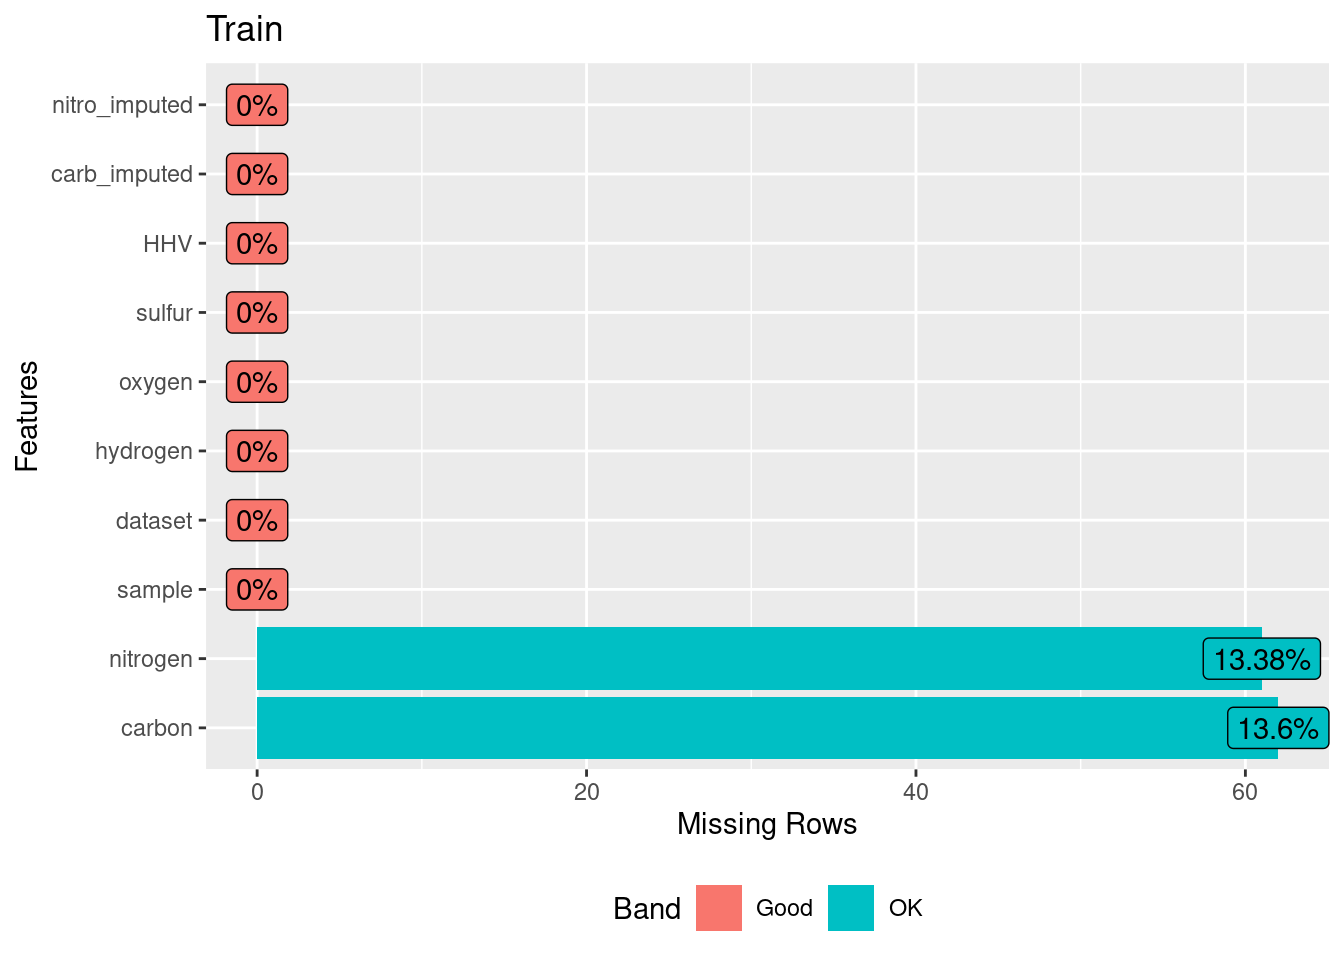
\includegraphics{amt22_03intro2mls2_files/figure-latex/unnamed-chunk-17-1.pdf}

\url{https://towardsdatascience.com/svm-and-kernel-svm-fed02bef1200}

\url{https://towardsdatascience.com/support-vector-machine-explained-8bfef2f17e71}

\url{https://medium.com/swlh/the-support-vector-machine-basic-concept-a5106bd3cc5f}

\url{https://towardsdatascience.com/unlocking-the-true-power-of-support-vector-regression-847fd123a4a0\#}:\textasciitilde:text=Support\%20Vector\%20Regression\%20is\%20a,the\%20maximum\%20number\%20of\%20points.

\url{https://www.mygreatlearning.com/blog/introduction-to-support-vector-machine/}

\url{https://www.robots.ox.ac.uk/~az/lectures/ml/lect3.pdf}

  \bibliography{book.bib,packages.bib}

\end{document}
